% The pantry in four moments (development case pantry_dev01, the same sources as fig_pantry.tex:
% DEMO.md section 4 and pantry_accounting.json). Target 40 kits by 13:40. 24 on the shelf, 16 in
% a partner pool at the same venue, 20 more in a late shipment that do not count as stock.
\documentclass[border=3pt]{standalone}
% Poster variant: the same figure with its type enlarged for reading at poster distance.
% Shared style of every Plan B figure (the deck, the poster and the documentation).
% Type is near-black and grey on white. UMB blue is the brand and the system. One warm accent
% marks tension only (the incoming message, the clock). Green marks only an accepted receipt or
% a met run. Square corners, thin rules, no shadows, no gradients.
\usepackage[T1]{fontenc}
\usepackage[scaled]{helvet}
\renewcommand{\familydefault}{\sfdefault}
\usepackage{tikz}
\usepackage{pgfplots}
\pgfplotsset{compat=1.18}
\usepackage{fontawesome5}
\hyphenpenalty=10000
\exhyphenpenalty=10000
\usetikzlibrary{arrows.meta,positioning,calc,fit,backgrounds}

% Colours
\definecolor{primary}{HTML}{08457E}   % UMB blue: the system, Plan B's own policy
\definecolor{primarysoft}{HTML}{E7EEF5}
\definecolor{accent}{HTML}{FF791F}    % tension only: the message, the gap, the one missed run
\definecolor{accentsoft}{HTML}{FFEBDC}
\definecolor{umbblue}{HTML}{005A8B}   % UMB blue: the three idea marks and structure
\definecolor{navy}{HTML}{132245}      % title bands, the receipt, the dark close
\definecolor{ground}{HTML}{EEF2F6}    % the light blue-grey ground behind white cards
\definecolor{ok}{HTML}{2E7D32}        % an accepted receipt, a met run
\definecolor{oksoft}{HTML}{E5F1E6}
\definecolor{ink}{HTML}{1F1F1F}
\definecolor{muted}{HTML}{6B6B6B}
\definecolor{quiet}{HTML}{9A9A9A}     % other policies, context
\definecolor{rulegrey}{HTML}{C4C4C4}
\definecolor{gridgrey}{HTML}{E4E4E4}
\definecolor{faint}{HTML}{F4F4F4}

\tikzset{
  >={Stealth[length=2.4mm,width=1.8mm]},
  every picture/.style={line cap=butt, line join=miter},
  % text styles
  hd/.style={font=\bfseries, text=ink, align=left},
  sub/.style={text=muted, align=left},
  % shapes: square or 1 pt corners, thin rules
  card/.style={draw=rulegrey, line width=0.5pt, fill=white, rounded corners=1pt, inner sep=5pt, align=left, text=ink},
  sys/.style={draw=primary, line width=0.8pt, fill=white, rounded corners=1pt, inner sep=5pt, align=center, text=ink},
  sysfill/.style={draw=primary, line width=0.8pt, fill=primary, rounded corners=1pt, inner sep=5pt, align=center, text=white},
  warm/.style={draw=accent, line width=0.8pt, fill=accentsoft, rounded corners=1pt, inner sep=5pt, align=left, text=ink},
  receipt/.style={draw=ok, line width=0.8pt, fill=oksoft, rounded corners=1pt, inner sep=5pt, align=left, text=ink},
  planned/.style={draw=muted, line width=0.6pt, dash pattern=on 3pt off 2pt, fill=white, rounded corners=1pt, inner sep=5pt, align=left, text=muted},
  % connectors
  link/.style={->, draw=muted, line width=0.6pt},
  syslink/.style={->, draw=primary, line width=0.9pt},
  oklink/.style={->, draw=ok, line width=0.9pt},
  warmlink/.style={->, draw=accent, line width=0.9pt},
  nextlink/.style={->, draw=muted, line width=0.6pt, dash pattern=on 3pt off 2pt},
}

% Charts: a real axis, few light gridlines, no frame on the top and right.
\pgfplotsset{
  planb/.style={
    axis line style={draw=muted, line width=0.5pt},
    tick style={draw=muted, line width=0.5pt},
    major tick length=3pt,
    tick label style={text=ink, /pgf/number format/assume math mode=true},
    label style={text=ink},
    title style={font=\bfseries, text=ink},
    grid style={draw=gridgrey, line width=0.4pt},
    every axis plot/.append style={line width=0.6pt},
    legend style={draw=none, fill=none, text=ink},
    legend cell align=left,
  },
}

% The three idea marks, the same in the deck, the poster and the report.
% 1 Check the fact (a magnifier), 2 Pick only what fits (a funnel that keeps what fits),
% 3 Leave a receipt (a receipt slip). Always in UMB blue unless the panel is navy.
\providecommand{\markcheck}{\faSearch}
\providecommand{\markfits}{\faFilter}
\providecommand{\markreceipt}{\faReceipt}
% The three points of "Why Plan B": safer shows the three marks together, more flexible a laptop,
% more personal a set of sliders.
\providecommand{\marksafer}{\faSearch\,\faFilter\,\faReceipt}
\providecommand{\markflexible}{\faLaptop}
\providecommand{\markpersonal}{\faSlidersH}

\begin{document}
\makeatletter
\renewcommand\tiny{\@setfontsize\tiny{7.2}{8.7}}
\renewcommand\scriptsize{\@setfontsize\scriptsize{10.2}{12.2}}
\renewcommand\footnotesize{\@setfontsize\footnotesize{11.6}{13.9}}
\renewcommand\small{\@setfontsize\small{13.0}{15.7}}
\renewcommand\normalsize{\@setfontsize\normalsize{14.5}{17.4}}
\renewcommand\large{\@setfontsize\large{17.4}{20.9}}
\renewcommand\Large{\@setfontsize\Large{20.9}{25.1}}
\makeatother
\normalsize

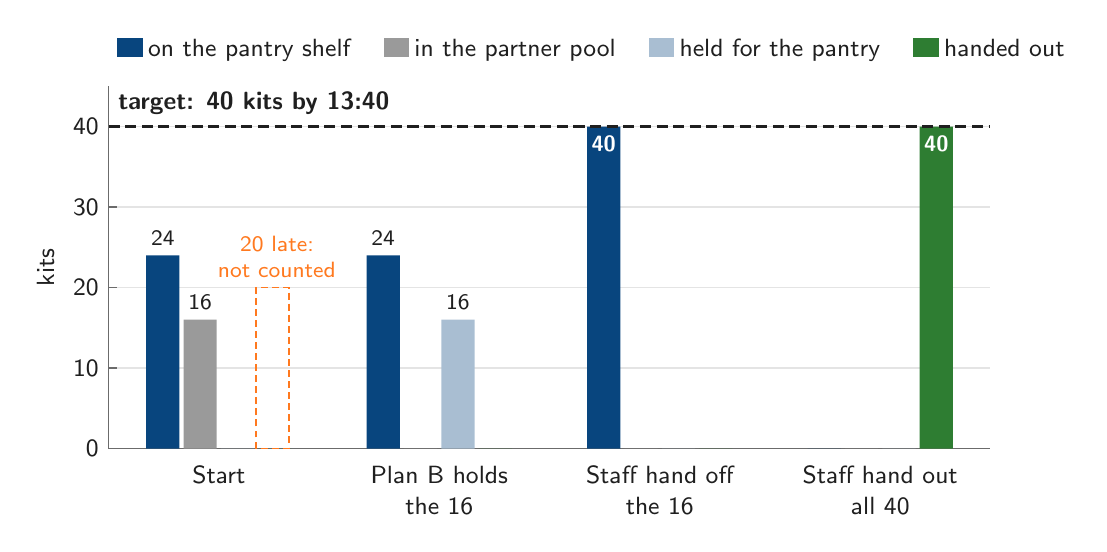
\begin{tikzpicture}[font=\small]
\begin{axis}[planb, scale only axis, width=11.2cm, height=4.6cm,
  ybar=1.5pt, bar width=12pt,
  ymin=0, ymax=45, ytick={0,10,20,30,40}, ymajorgrids,
  axis x line*=bottom, axis y line*=left, xtick style={draw=none},
  xtick={1,2,3,4}, xmin=0.5, xmax=4.5,
  xticklabels={{Start},{Plan B holds\\the 16},{Staff hand off\\the 16},{Staff hand out\\all 40}},
  xticklabel style={align=center, text=ink},
    ylabel={kits},
  legend style={at={(0.0,1.04)}, anchor=south west, legend columns=4, /tikz/every even column/.append style={column sep=10pt}},
  legend image code/.code={\fill[#1] (0cm,-0.1cm) rectangle (0.32cm,0.14cm);},
  clip=false]
  \addplot[fill=primary, draw=none] coordinates {(1,24) (2,24) (3,40) (4,0)};
  \addlegendentry{on the pantry shelf}
  \addplot[fill=quiet, draw=none] coordinates {(1,16) (2,0) (3,0) (4,0)};
  \addlegendentry{in the partner pool}
  \addplot[fill=primary!35, draw=none] coordinates {(1,0) (2,16) (3,0) (4,0)};
  \addlegendentry{held for the pantry}
  \addplot[fill=ok, draw=none] coordinates {(1,0) (2,0) (3,0) (4,40)};
  \addlegendentry{handed out}
  % the target
  \draw[ink, line width=0.8pt, dash pattern=on 4pt off 2pt] (axis cs:0.5,40) -- (axis cs:4.5,40);
  \node[anchor=south west, text=ink, font=\small\bfseries] at (axis cs:0.5,40.3) {target: 40 kits by 13:40};
  % value labels (the bars are 12 pt wide with 1.5 pt between them, four bars per group)
  \node[anchor=south, text=ink, font=\footnotesize] at ([xshift=-20.25pt]axis cs:1,24) {24};
  \node[anchor=south, text=ink, font=\footnotesize] at ([xshift=-6.75pt]axis cs:1,16) {16};
  \node[anchor=south, text=ink, font=\footnotesize] at ([xshift=-20.25pt]axis cs:2,24) {24};
  \node[anchor=north, text=white, font=\footnotesize\bfseries] at ([xshift=-20.25pt]axis cs:3,40) {40};
  \node[anchor=south, text=ink, font=\footnotesize] at ([xshift=6.75pt]axis cs:2,16) {16};
  \node[anchor=north, text=white, font=\footnotesize\bfseries] at ([xshift=20.25pt]axis cs:4,40) {40};
  % the late shipment: not stock
  \draw[accent, line width=0.7pt, dash pattern=on 2.5pt off 1.5pt] ([xshift=13.5pt]axis cs:1,0) rectangle ([xshift=25.5pt]axis cs:1,20);
  \node[anchor=south, text=accent, font=\footnotesize, align=center] at ([xshift=21pt]axis cs:1,20) {20 late:\\not counted};
\end{axis}
\end{tikzpicture}
\end{document}
